\chapter{Gravity and Geometry}
\label{chapter:gravity}

\section{Introduction}

Previously we have described the force of gravity on an object by a
field model.  In this Newtonian model, masses cause gravitational fields and
these fields act on other masses to cause forces.
    
In this chapter we examine another model of gravity which is
Einstein's explanation in terms of curved spacetime.  In this model
masses cause spacetime to be curved and other masses, moving in
`straight' lines in this curved spacetime, seem to accelerate relative
to the source mass.  As described succinctly by John A. Wheeler,
the leading spokesman for Einstein's theory of gravity: 

\begin{quote}
Mass tells spacetime how to curve;  spacetime tells mass how to
move.
\end{quote}

We begin by looking again at the concept of the invariant spacetime
interval.  We present the modifications of the interval that Einstein
introduced to account for the effects of gravity.  This leads us to
examine how the gravitational effects of a spherical mass (like
planets and stars) show up in clock rates and the measurement of
distances.
    
We also develop the idea of curved space and describe how one might
determine whether the three-dimensional space we live in is curved.
We apply this idea to the curvature of spacetime to examine how a
particle moves in curved spacetime and present an unusual principle
called the principle of maximum proper time which governs how an
object moves in the presence of a gravitational field.

\section{The Interval Revisited}

In developing his conception of gravity as a manifestation of curved
spacetime, Einstein sought to extend his notion of invariance from
special relativity.  Recall that for special relativity all
\textit{inertial} reference frames were treated as equally valid for
describing physics.  In 1915, Einstein created the theory of general
relativity, removing the inertial frame restriction: \textit{all
  arbitrarily} moving reference frames were to be equally valid.  This
enabled him to include gravity into spacetime physics.

Recall that in Sec.~\ref{sec:spacetime_intervals} we introduced the
spacetime interval $I^2$ of special relativity, defined by
\begin{equation}
I^2 = (c\Delta t)^2 - (\Delta x)^2.
\end{equation}     
The interval was shown to be invariant: observers in any inertial
reference frame would calculate the same value for the interval
separating any given pair of events.  

%%%%%%%%%%%%%%%%%%%%%%%%%

Also recall that when $I^2$ is
positive the interval $I$ is time-like. In some frame the two events
happen at the same location, so $\Delta x=0$
and the interval, in fact, measures proper time $\Delta\tau$:
\begin{equation} 
   \Delta\tau^2  = I^2/c^2 \qquad\text{(proper time for timelike interval)}
   \label{eq:proper_time}
\end{equation}
On the other hand, when $I^2$ is negative, we are dealing with a
spacelike interval.  In some frame the two events are simultaneous
($\Delta t=0$) and $\Delta x$ represents a length measurement.  It is
convenient to introduce $\Delta s$, the proper distance, by
\begin{equation}
 \Delta s^2 = -I^2 > 0 \qquad\text{(proper distance for spacelike interval)}.
 \label{eq:proper_distance}
\end{equation}

%%%%%%%%%%%%%%%%%%%%%%%%%%%%%%%%%%%%

\begin{figure}[tbp]
\begin{center}
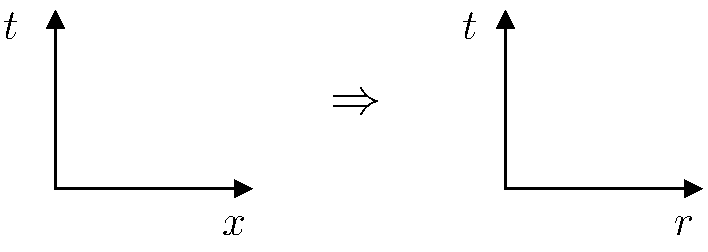
\includegraphics[width=2.5in]{gravity_and_geometry/coordinates.pdf}
\end{center}
\caption{Cartesian to polar coordinates}
\label{fig:cartesian_to_spherical}
\end{figure}

Now let's work on generalizing the interval $I^2$ to include the effects of
gravity.  The first thing to do is convert from Cartesian to polar
coordinates, shown in Fig.~\ref{fig:cartesian_to_spherical}, as
these will be more appropriate to describe spacetime in the presence
of spherically symmetric masses, like Earth, stars, or black holes.
Here ``$r$'' is a radial coordinate: it decreases or increases as you
move toward or away from the given spherical mass.  The interval
expressed in these coordinates, not surprisingly, takes the form
\begin{equation}
I^2 =  (c\Delta t)^2 - \Delta r^2
\label{eq:flat_space_spherical}
\end{equation}
when motion along only the radial direction is considered.

Next, let's see how Einstein includes the effects of gravity in the
invariant spacetime interval.  How is it that ``mass tells spacetime
how to curve''?  The full answer is very hard, far beyond the scope of
this course: solve a set of nasty coupled nonlinear differential
equations!  But for the case of intervals in the spacetime outside a
spherical mass, the result is surprisingly simple.
Eq.~(\ref{eq:flat_space_spherical}) becomes
\begin{equation}
  I^2 = \biggl(1-\frac{2GM}{c^2 r}\biggr)(c\Delta t)^2-
  \biggl(1-\frac{2GM}{c^2 r}\biggr)^{-1}\Delta r^2. 
\label{eq:schwarzschild_metric}
\end{equation}
Here ``$M$'' is the mass of the central body, and $G$ is Newton's
universal gravitation constant.

The appearance of the coefficients $(1-\frac{2GM}{c^2r})$ and
$(1-\frac{2GM}{c^2r})^{-1}$ in the general relativistic expression for
the spacetime interval tells you that we're now dealing with curved
spacetime.  The presence of a nearby mass curves spacetime!  

Let's explore how these gravity-related factors lead to the warping of
time and space.

\section{Gravity's Effect on Clock Rates}

An example will show how clock rates are affected by the curvature of
spacetime.  Consider two clocks, clock $A$ parked near a large mass,
and clock $B$ parked very far away.  Note that both clocks are at
rest: there is NO relative motion.  Yet general relativity predicts
that the clocks still run at different rates.

Take a clock located at coordinate $r$, with events 1 and 2 as
successive ticks on the clock.  Starting
from Eq.~(\ref{eq:schwarzschild_metric}), we insert the
condition that the clock is stationary ($\Delta r=0$), and use the
result that the interval measures proper time $\Delta\tau$ to get
\begin{equation}
  \Delta\tau^2 = \biggl(1-\frac{2GM}{c^2 r}\biggr)\Delta t^2.
\label{eq:clock_rates}
\end{equation}
This expression requires careful interpretation: $\Delta\tau$ represents
the actual time measured by the clock at coordinate $r$.  So what is
$\Delta t$?

Since clock $B$ is very far away (say $r_B\to\infty$), so that
$\frac{2GM}{c^2r_B}\to 0$, then for $B$
Eq.~(\ref{eq:clock_rates}) becomes
\begin{equation}
  \Delta \tau_B^2 = (1-0)\Delta t^2 = \Delta t^2 \quad\text{or}\quad
  \Delta\tau_B = \Delta\tau.
\end{equation}
This shows that $\Delta t$ can be understood as the proper time as
recorded on far-away clocks.

\begin{figure}[tbp]
\begin{center}
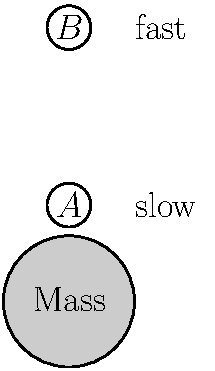
\includegraphics[width=1in]{gravity_and_geometry/clocks.pdf}
\end{center}
\caption{Low clocks are slow clocks!}
\label{fig:clocks}
\end{figure}

Now consider clock $A$, say at rest at radial location $r_A$.  Similar
to the above calculation we find
\begin{equation}
 \Delta\tau_A = \biggl( 1 - \frac{2GM}{c^2 r_A}\biggr)^{1/2} \Delta t
    = \biggl( 1 - \frac{2GM}{c^2 r_A}\biggr)^{1/2} \Delta\tau_B.
\label{eq:low_clock}
\end{equation}
Since $(1-\frac{2GM}{c^2r})^{1/2} < 1$, we see that
$\Delta\tau_A<\Delta\tau_B$.
This shows that clocks near a mass record \textit{less} elapsed proper
time than those far away.  As illustrated in Fig.~\ref{fig:clocks}, a
nice mnemonic is ``Low clocks are slow clocks''.

\begin{example}{Clocks on the Earth's Surface.}
How much slower does a clock at sea level run than one very far away from
Earth?
\solution

Use Eq.~(\ref{eq:low_clock}), with $M=5.97\times 10^{24}\units{kg}$
and $r_A=R_E = 6.37\times 10^{6}\units{m}$
\begin{align}
 \Delta\tau_A &= \biggl(1-\frac{2\times 6.67\times 10^{-11}\times
   5.97\times 10^{24}}{(3.00\times 10^{8})^2 \times 6.37\times 10^{6}}
\biggr)^{1/2}\Delta\tau_B   \nonumber\\
   &= (1-1.39\times 10^{-9})^{1/2}\Delta\tau_B \nonumber\\
   &\approx (1 - 6.95\times 10^{-10}) \Delta\tau_B.
\end{align}
A useful way to express this result is the rate at which clock $A$
gets behind:
\begin{equation}
  \Delta\tau_B - \Delta\tau_A = \Delta\tau_B -
     (1 - 6.95\times 10^{-10}) \Delta\tau_B = 
6.95\times 10^{-10} \Delta\tau_B. 
\end{equation}
Thus clock $A$ falls behind clock $B$ an amount $6.95\times 10^{-10}$
seconds every second.  Thus, for clock $A$ to get behind clock $B$ by
one second, it takes 
\begin{equation}
\frac{1}{6.95\times 10^{-10}} \text{seconds} = 1.44\times
10^9\units{s}   \approx 46\units{yr}.
\end{equation}
\end{example}
We don't notice these time effects much near Earth, but these small
difference are essential to be accounted for in the design and
operations of GPS devices.  For a more dramatic example, see Problem
\ref{prob:neutron_star_time}.
 
\section{Curved Spacetime}
     
We now need to give a careful definition of the radial coordinate $r$.
We begin with an example in ordinary three-dimensional space.  Imagine
drawing two large circles on the earth with the north pole as the
common center (see Fig.~\ref{fig:sphere}).  Let $\Delta s$ be the distance
between one circle and the other, measured along the earth's surface
as we walk out from the north pole.  If we were sphere-dwellers who
lived entirely in 2-dimensions, that is, on the surface of the earth,
and knew nothing about a 3$^{\rm rd}$ dimension (up or down), we could
{\em define} the radial
coordinates, $r_1$ and $r_2$, in terms of the circumferences of the
two circles, by
\begin{equation}
C_1 = 2\pi r_1\mbox{\hspace{.25in}and\hspace{.25in}}C_2 = 2\pi r_2.
\label{eq:circumference}
\end{equation}
The actual radii of the circles, $r_1$ and $r_2$, are shown in
Fig.~\ref{fig:sphere}; they clearly are not measured along the surface
of the earth.  But these radii are not available for direct
measurement by the sphere-dwellers; they must \textit{calculate} the
radii using Eq.~(\ref{eq:circumference}).
     
\begin{figure}[tbp]
\begin{center}
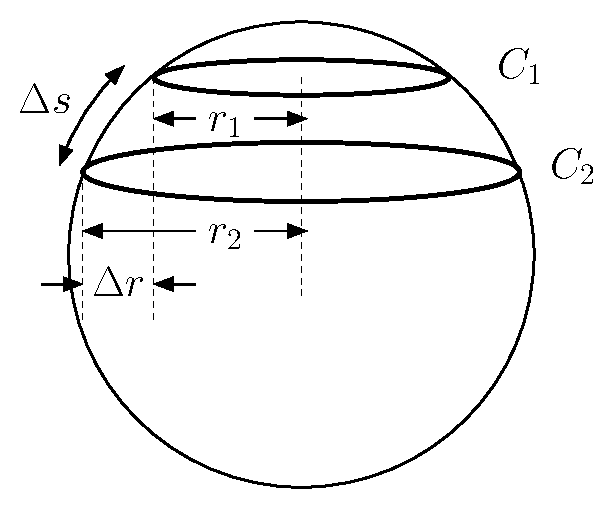
\includegraphics[width=2in]{gravity_and_geometry/sphere.eps}
\end{center}
\caption{Two concentric circles drawn on a sphere.}
\label{fig:sphere}
\end{figure}
     
If we lived on a flat space, such as a flat piece of paper, the radial
coordinates $r_1$ and $r_2$ would be related by
\begin{equation}
\Delta r = r_2 - r_1 = \Delta s \mbox{\hspace{0.5in}(flat space
  expectation)},
\label{eq:flat}
\end{equation}
where $\Delta s$ is the shortest distance between the circles measured
along the paper.  But when the circles are actually drawn on the
curved surface of the earth, $r_2$ is larger than $r_1$ by the amount
$\Delta r$, which is less than $\Delta s$.
     
We humans, who can comprehend the spherical nature of the earth's
surface, can understand this deviation from flat-space geometry by
studying Fig.~\ref{fig:sphere}, where the actual difference in radius,
$\Delta r$, between the two circles on the earth is clearly smaller
than $\Delta s$.  Thus, on a sphere, the flat-space expectation of
Eq.~(\ref{eq:flat}) is incorrect.  We can therefore use
Eq.~(\ref{eq:flat}) in an experimental test, performed entirely on the
surface of the earth, to determine whether that surface is curved or
flat.
     
The test requires that we measure the circumferences of the two
circles and the distance $\Delta s$ between them.  Then we must divide
each circumference by $2\pi$ to get the radial coordinate, substitute
these calculated values for $r_1$ and $r_2$, along with the measured
$\Delta s$, into Eq.~(\ref{eq:flat}) and check for equality.  If we
get equality then the surface is flat.  If $\Delta s$ is larger than
$r_2-r_1$, then the surface is curved like a sphere or a bowl.  (If
$\Delta s$ is smaller, the surface is curved like a saddle.)

\begin{figure}[tbp]
\begin{center}
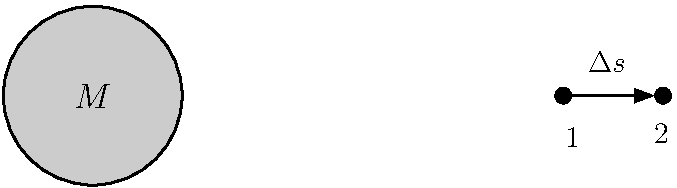
\includegraphics[width=3.5in]{gravity_and_geometry/grav-photon.pdf}
\end{center}
\caption{An outward displacement $\Delta s$ in the gravitational field
  of a star.}
\label{fig:grav-photon}
\end{figure}
     
Now let's consider the region around a star as shown in
Fig.~\ref{fig:grav-photon}.  We ask whether the space around the star
is curved.  How can we tell?  We begin by drawing two circles centered
on the star, $C_1$ and $C_2$ in Fig.~\ref{fig:concentric}.  We then
measure their circumferences with meter sticks (which have been
properly calibrated with clocks and light pulses) and calculate $r_1$
and $r_2$.  We also measure the distance $\Delta s$, by laying meter
sticks radially along a path from $C_1$ to $C_2$.  Then to test
whether space is curved or flat, we substitute our measurements into
Eq.~(\ref{eq:flat}).  If Eq.~(\ref{eq:flat}) is satisfied, then space
is flat; otherwise it is curved.
         

\begin{figure}[t]
\begin{center}
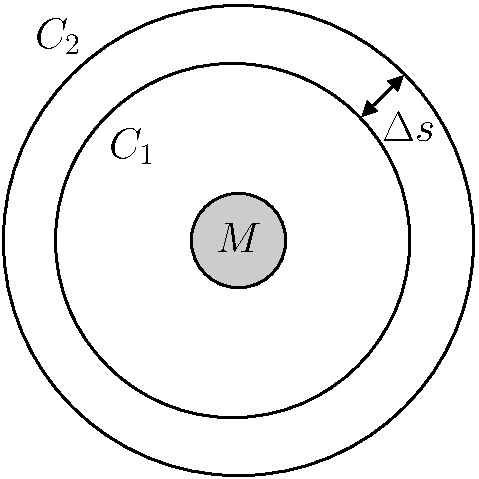
\includegraphics[width=1.8in]{gravity_and_geometry/concentric.pdf}
\end{center}
\caption{Two concentric circles drawn around a star of mass $M$.}
\label{fig:concentric}
\end{figure}
     
When we do this experiment (say with radar ranging around the sun) we
find that actual measurements of phenomena occurring near the sun
indicate that $\Delta s$ is, in fact, slightly larger than $\Delta r$.
Thus Eq.~(\ref{eq:flat}) is {\em not} satisfied, and the space around
the sun is curved like a bowl.  The source of the curvature is the
mass $M$ of the sun.  It's like placing a large mass on a rubber
sheet; the added mass distorts and curves the sheet so that nearby
smaller masses are attracted to it.  Near a black hole, the curvature
effect is quite pronounced.  Figure~\ref{fig:curved-space} shows a
popular representation of the curved space near a black hole.
     
\begin{figure}[tbp]
\begin{center}
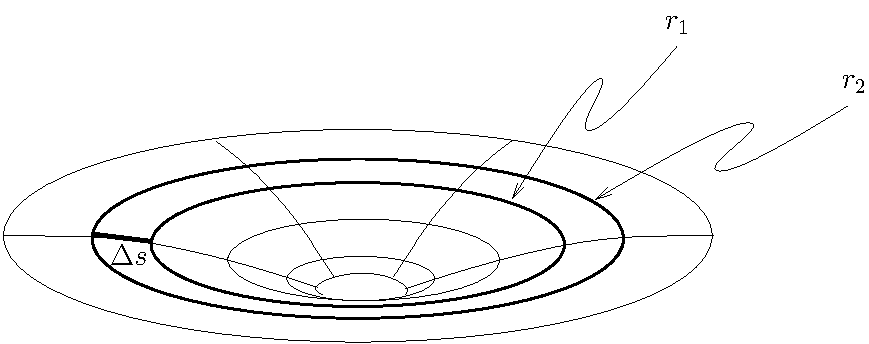
\includegraphics[width=4in]{gravity_and_geometry/black-hole.pdf}
\end{center}
\caption{Curved space near a black hole.  The distance $\Delta s$ measured
radially along the surface between circles of radial coordinate  $r_1$ 
and $r_2$ is larger than their  difference $\Delta r$.}
\label{fig:curved-space}
\end{figure}
     
     
It's time to get quantitative.  Can Einstein's conception of curved
spacetime near the sun tell us that $\Delta s$ is bigger than $\Delta
r$, and by how much? We would like to consider a snapshot of the space around the sun; that
is locate the two points at the \textit{same time}.  Thus set $\Delta
t=0$ in
Eq.~(\ref{eq:schwarzschild_metric}), and use
$\Delta s^2=-I^2$ to get
\begin{equation}
  \Delta s = \biggl(1-\frac{2GM}{c^2 r}\biggr)^{-1/2}\Delta r.
\label{eq:schwarzschild_metric_iv}
\end{equation}
Since $(1-\frac{2GM}{c^2r})^{-1/2} > 1$ for any $M>0$ and $r<\infty$
we have that $\Delta s>\Delta r$ near any mass --- the space near
stars and planets is curved like a bowl!

\begin{example}{}
How curved is space near the sun?
\solution
Use Eq.~(\ref{eq:schwarzschild_metric_iv}) with $M=M_\text{sun}=
1.99\times 10^{30}\units{kg}$ and $r=R_\text{sun}=6.96\times
10^{8}\units{m}$.
\begin{align}
\Delta s &= \biggl(1-\frac{2\times 6.67\times 10^{-11}\times 1.99\times
  10^{30}}{(3.00\times 10^{8})^2\times 6.96\times
  10^8}\biggr)^{-1/2}\Delta r \nonumber\\
 &= (1-4.24\times 10^{-6})^{-1/2}\Delta r \nonumber\\
 &= 1.0000021\,\Delta r.
\end{align}
That's not looking very curved, but it is big enough to direct the
motion of all the planets in their orbits about the sun!
\end{example}


\section{Law of Motion for a Freely Falling Body}
     
We have described the way matter tells spacetime how to curve; now
let's address the second half of Wheeler's quote: how does spacetime tell
matter how to move?  The answer is the \textit{principle of maximum
proper time}, which can be stated as follows:
\begin{quote}
  An object begins at
coordinate $x_i$ at time $t_i$ and its trajectory ends at coordinate
$x_f$ at time $t_f$.  Consider all the possible paths
that this object could take, and determine the proper time elapsed for
each path.  The path that provides the longest proper time is the
`natural' motion of the object, and corresponds to the path taken.
\end{quote}

Let's illustrate this with a couple of examples.
Imagine taking a trip, in gravity-free spacetime, from the point $x =
0$, $t = 0$ to the point $x = 0$, $t = 1\units{s}$.  Not a very adventurous
trip, to be sure!  Since there is no gravity around, Newton's first law
says the `natural' motion will be for the object to simply stay at the
origin, and of course $1\units{s}$ of proper time would elapse on this
trip. 

But there are other ways to consider making the trip (see
Fig.~\ref{fig:trip}).  For example you could take off at some high
speed, say $v = 0.6 c$ for half a second (in the rest frame) and
travel about 0.3\units{lt-s} and then suddenly reverse direction and
travel for another half second back to $x = 0$ at a velocity of $-0.6
c$.  With this hyperactive approach the time elapsed on your watch
(proper time) will be only
\begin{equation}
\Delta t_{\rm proper} = \Delta t \sqrt{1 - v^2/c^2} = 
      1.0 \times \sqrt{1 - 0.6^2} = 0.8\, \mbox{s},
\label{eq:deltatnograv}
\end{equation}     
which is less than the $1.0\units{s}$ of the stationary path.
Of all the ways of making the trip, the one taken at zero velocity
will give the longest proper time.  This obviously physical
`natural' path indeed is the one with maximum proper time.
        
\begin{figure}[h]  
\begin{minipage}[t]{5.0cm}
\begin{center}
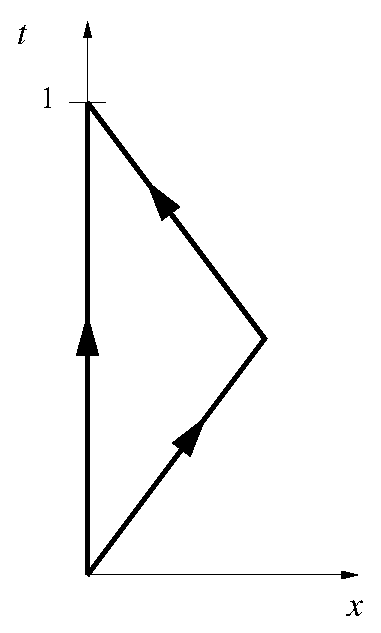
\includegraphics[height=6cm]{gravity_and_geometry/trip.eps}
\caption{Two ways of taking a spacetime trip.}
\label{fig:trip}
\end{center}   
\end{minipage}
\hfill
\begin{minipage}[t]{6.3cm}
\begin{center}
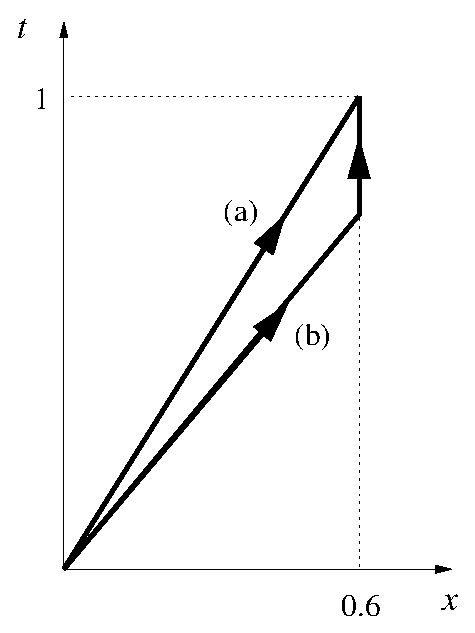
\includegraphics[height=6cm]{gravity_and_geometry/trip2.eps}
\caption{Two ways of taking a different spacetime trip.}
\label{fig:trip2}
\end{center}
\end{minipage}
\end{figure}

For another example, suppose we want to go from the point $x = 0$, $t
= 0$ to the point $x = 0.6\units{lt-s}$, $t = 1\units{s}$.  Since
there is no gravity, the velocity should be constant, and we should
expect that the way to take the trip in the greatest proper time is to
go at a constant velocity $v = 0.6 c$, shown as route (a) in
Fig.~\ref{fig:trip2}.  We already know that the proper time for this
constant velocity trip is $(1 -0.6^2)^{1/2} = 0.8\, \mbox{s}$.  Is this
the maximum proper time?
        
Figure \ref{fig:trip2} shows an alternate route to get to $x =
0.6\units{lt-s}$, $t = 1\units{s}$, labeled as path (b).  In homework
problem \ref{prob:trip}, you will calculate the proper time for this
route.  What you should find is that the total proper time is less for
the two-step trip, route (b), than for the 0.8 second `natural' trip at a
single velocity, route (a).  Once again, the obviously physical
`natural' motion corresponds to maximum proper time.

This same principle works in curved spacetime.  The path between two
events actually taken by a freely falling body is that path that
MAXIMIZES the elapsed proper time.  This rule leads to the
``straightest'' possible path through the curved spacetime, and
answers the question:  How is it that ``spacetime tells mass how to
move''?

Now imagine the motion of some object in the curved space around a
mass $M$.  Maximizing proper time requires a balance between
maximizing clock rates (so avoiding going into the center, where
``lower is slower'') and minimizing distance.  The full calculation is
beyond the scope of this course, but result reproduces the effect we
normally think of as a gravitational force: the trajectory is bent by
the presence of the central mass $M$.  But note that this bending
would affect any object passing by, even something massless like
light!  This is why light bends around large mass stars or galaxies
(see Fig.~\ref{fig:light-bent-by-curved-space}), which is one of the
striking predictions of general relativity.

\begin{figure}[b]
\begin{center}
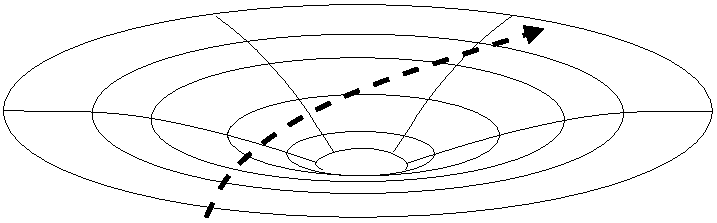
\includegraphics[width=3in]{gravity_and_geometry/black-hole-bends-light.pdf}
\end{center}
\caption{Light being bent by curved space near a black hole.}
\label{fig:light-bent-by-curved-space}
\end{figure}



\begin{figure}[t]
\begin{center}
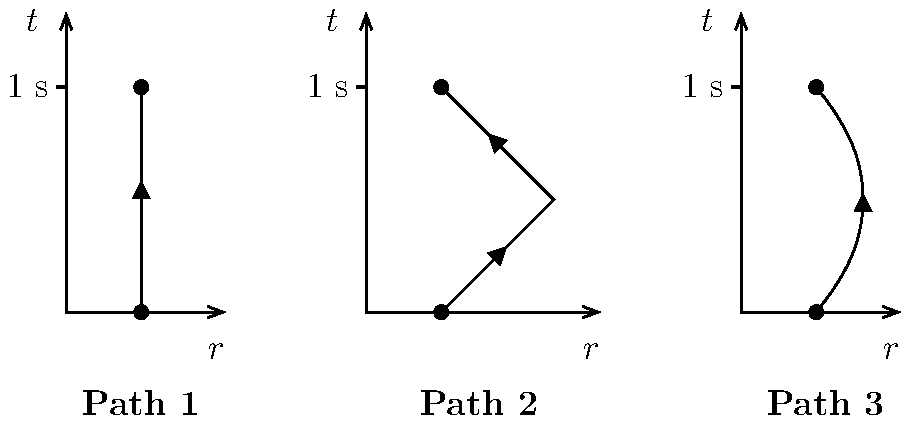
\includegraphics[width=4in]{gravity_and_geometry/trajectory.pdf}
\end{center}
\caption{Trajectories}
\label{fig:trajectories}
\end{figure}
     
\section{Summary}

Taken together, the curved spacetime produced by mass $M$ and the
principle of maximum proper time for trajectories is able to explain
all the phenomena that we normally think of as Newtonian gravity.
The predictions are in fact exactly the same as Newtonian gravity whenever
the curvature is not large.  Deviations from
Newtonian gravity have been measured in the orbit of Mercury, and the 
bending of light near the Sun.

But how can general relativity explain the simple motion of a ball
tossed in the air?  Throw a ball straight up and catch it
one second later at the same original height.  What is the ``naturally
chosen'' path through spacetime that maximizes proper time?  We have
just seen that, because of time dilation, paths that speed up, slow
down, or reverse direction tend to \textit{decrease} proper time.  On
the other hand, we've learned that clocks at higher altitudes measure
\textit{more} elapsed proper time than those at lower altitudes.  So
now consider these three paths, shown in Fig.~\ref{fig:trajectories}:

\begin{description}
\item[Path 1] The ball stays just above your hand the whole time.  No
  speeding to decrease proper time --- BUT also not taking advantage of
  increasing proper time by going high where clocks run faster.   Not
  the best.

\item[Path 2] Zoom high at almost light-speed, zoom back down.  This
  gets the ball high where clocks run fast, but time dilation at near
  light speed means almost no elapsed proper time!  No good.

\item[Path 3] Spend most of the trip at a higher place where proper
  time elapses rapidly.  But don't go very fast or change speed
  quickly, so the time dilation is not too severe.
\end{description}
        
Result: Best path for maximizing proper time is parabolic motion ---
fast up, slow and stop smoothly at the top, faster on the way down.
This is the motion we actually observe!



\newpage     

\section*{Problems}
\markright{PROBLEMS}

\begin{problem}
  Refer to Fig.~\ref{fig:sphere}.  Suppose $C_1$ is the $50^\circ$
  north latitude circle on the earth, and $C_2$ is the $40^\circ$
  north latitude circle on Earth.  The measured circumferences are
  $C_1 = 25850\, \mbox{km}$ and $C_2 = 30800\, \mbox{km}$.
  \begin{enumerate}
  \item Determine $r_1$, $r_2$ and $\Delta r$.
  \item Determine $\Delta s$ as a direct measurement on the earth's surface
    of the distance between the $40^\circ$ and $50^\circ$ latitude
    circles.  Compare your result to $\Delta r$.
  \item Explain how you could use your results to convince a member of
    the Flat Earth Society that the earth's surface is actually
    curved.
  \end{enumerate}
  \label{prob:sphere}
\end{problem}


\begin{problem}
  Consider clock $C$ on the surface of a neutron star, and clock $D$
  far away.  How do their rates compare?  How much time elapses on
  clock $D$ before clock $C$ is one second behind?  (The mass and
  radius of the neutron star are $2\times 10^{30}\units{kg}$ and
  $10\units{km}$, respectively.)
  \label{prob:neutron_star_time}
\end{problem}

\begin{problem}
  For the same neutron star as in
  Problem~\ref{prob:neutron_star_time}, calculate the height above
  the surface for which the circumference of a circle concentric with
  the star is $2\pi\times 10.001\units{km}$.
  \label{prob:neutron_star_space}
\end{problem}


\begin{problem}
  Following path (b) in Fig.~\ref{fig:trip2} means you go at $v =
  0.8c$ for the first leg, and $v = 0$ for the next.  Calculate the
  $t$-coordinate at the junction point; then determine the proper time
  for each leg and add them to get the total proper time.  Compare to
  the $0.8\, \mbox{s}$ of the direct route.
  \label{prob:trip}
\end{problem}

